
% Este documento LaTeX fue dise�ado por profesores  del Departamento de Matem�ticas 
% de la Universidad de Antioqua (http://ciencias.udea.edu.co/). Usted puede modificarlo
% y personalizarlo a su gusto bajo los t�rminos de la licencia de documentaci�n libre GNU.
% http://es.wikipedia.org/w/index.php?title=Licencia_de_documentaci%C3%B3n_libre_de_GNU&oldid=15717448

\documentclass[serif,9pt]{beamer}
\setbeamertemplate{navigation symbols}{}

\usetheme{Warsaw}

%\documentclass[serif,9pt]{beamer}
%\usepackage[T1]{fontenc} % Needed for Type1 Concrete
%\usepackage[charter]{mathdesign}

%\usepackage[pdftex]{graphicx}

\usepackage[latin1]{inputenc}
\usepackage[spanish]{babel}

\beamersetuncovermixins{\opaqueness<1>{25}}{\opaqueness<2->{15}}

\begin{document}
\title[Trabajo fin de grado]{WebGL Based 3D Dashboard for Tracking Software Development}  
\author{Adri�n Alonso Barriuso}

\institute[Universidad Rey Juan Carlos]{%
  ESCUELA T�CNICA SUPERIOR DE INGENIER�A DE TELECOMUNICACI�N\\
  Universidad Rey Juan Carlos}
\date{2016}

\logo{
\includegraphics[scale=0.1]{logo_vect}} 


\begin{frame}
\titlepage
\end{frame}

\begin{frame}\frametitle{Contenido}\tableofcontents
\end{frame} 

\section{Introducci�n} 

\subsection{Descripci�n del problema}

\begin{frame}\frametitle{Dashboards y seguimiento de desarrollo de software } 

 Un \textbf{dashboard} es una interfaz de ususario que nos permite manejar y gestionar un tipo determinado de software o de hardware. En nuestro caso trabajamos con dashboards de visualizaci�n de datos de desarrollo de software.
Algunos ejemplos de dashboards y de librer�as para la visualzacion de datos basadas en software libre son:
 
\begin{itemize}

\item \textbf{Kibana}

\item \textbf{Freeboard}

\item \textbf{dc}

\end{itemize}

\end{frame}

\begin{frame}\frametitle{Kibana} 

\begin{figure}
  \centering
  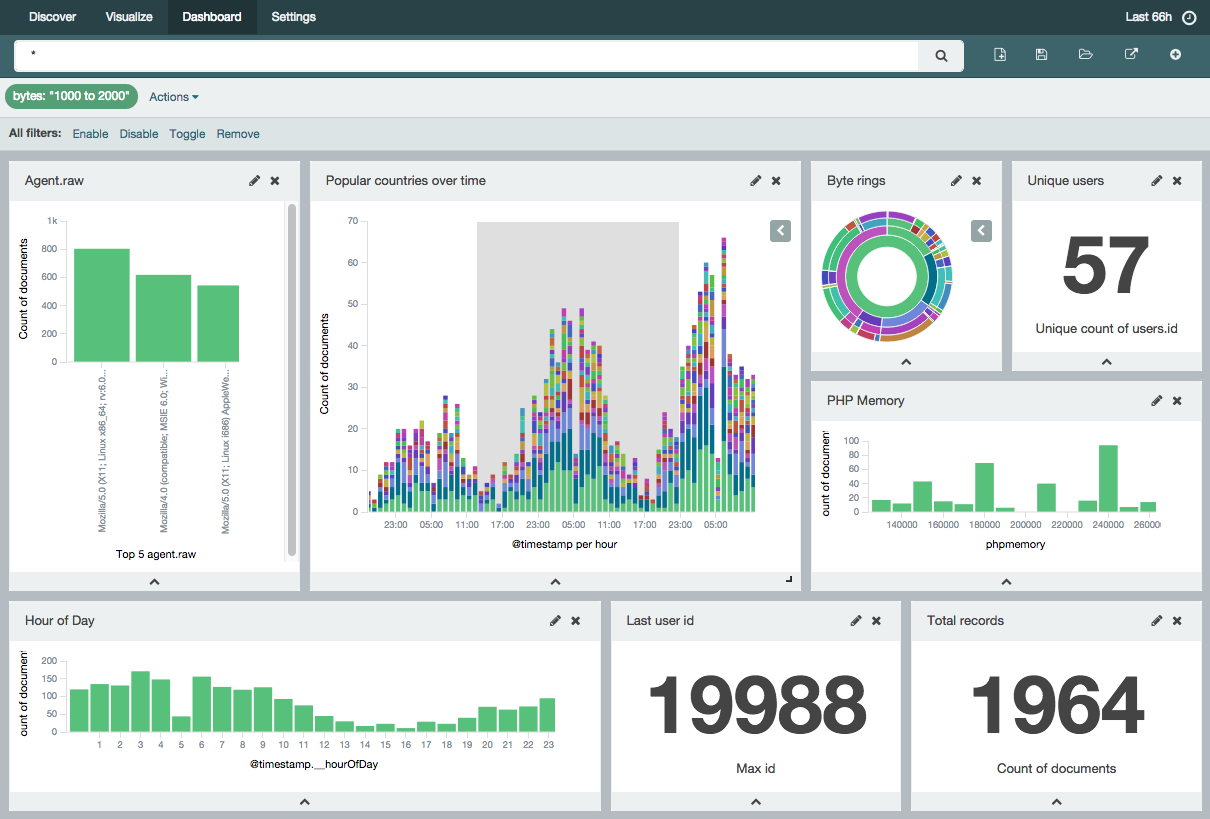
\includegraphics[width=9cm, keepaspectratio]{kibana}
  \caption{ejemplo de Kibana}
  \label{fig:car}
\end{figure}
\end{frame}

\begin{frame}\frametitle{Freeboard} 

\begin{figure}
  \centering
  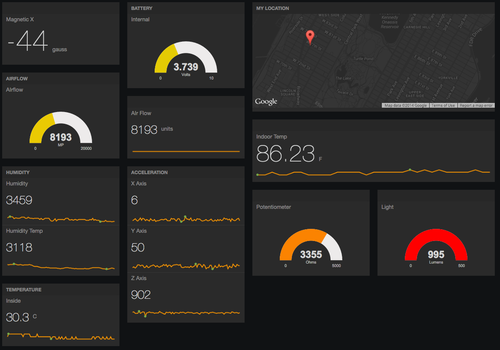
\includegraphics[width=8cm, keepaspectratio]{freeboard}
  \caption{Ejemplo de freeboard}
  \label{fig:car}
\end{figure}

\end{frame}

\begin{frame}\frametitle{dc} 

\begin{figure}
  \centering
  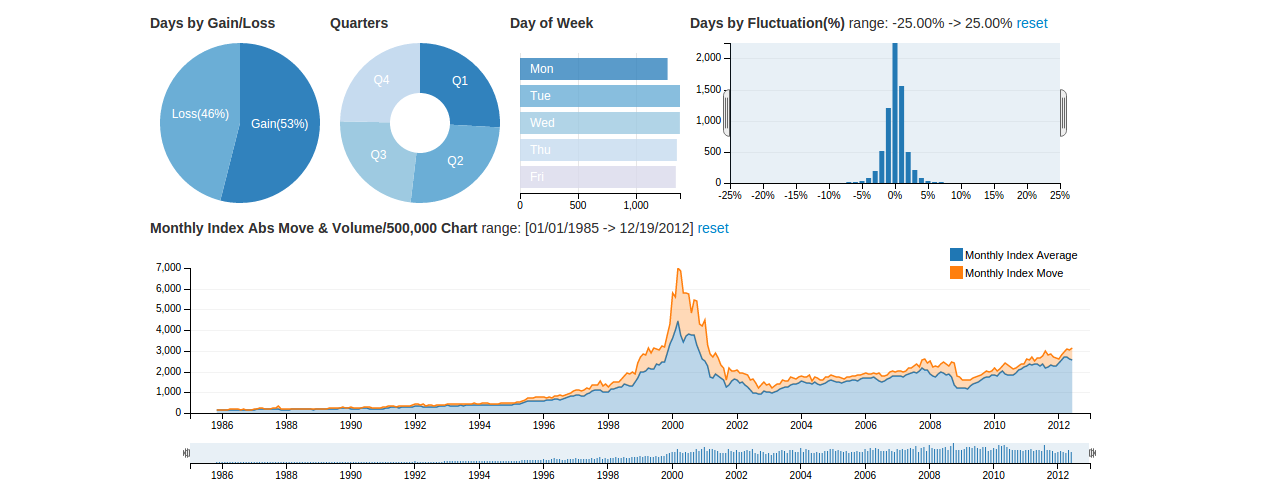
\includegraphics[width=12cm, keepaspectratio]{dc_example1}
  \caption{ejemplo de uso de dc.js}
  \label{fig:car}
\end{figure}

\end{frame}

\begin{frame}\frametitle{Dashboards en 2D } 

\begin{exampleblock}{Ventajas}
\begin{enumerate}
\item Simplicidad de representaci�n.
\item No requieren aceleraci�n gr�fica.
\item Impacto m�nimo en el rendimiento.
\end{enumerate}
\end{exampleblock}

\begin{alertblock}{Inconvenientes}
\begin{enumerate}
\item No se pueden representar gr�ficos con mas de 2 dimensiones, por razones obvias.
\item Las posibilidades de visualizaci�n y colocaci�n son limitadas.
\end{enumerate}
\end{alertblock}

\end{frame}


\subsection{Objetivo principal}
\begin{frame}
\frametitle{Objetivo principal} 

Crear una librer�a que nos permita crear visualizaciones y filtrar datos de desarrollo de software en 3D, dentro de cualquier navegador.
\begin{block}{Requisitos}
\begin{enumerate}
\item Conseguir una interfaz y funcionalidad tan parecidos a los de dc.js como sea posible.
\item Tener varios tipos de gr�ficas y ser capaces de filtrar.
\item Utilizar un framework de webGL
\item Respuesta r�pida de los filtros.
\item Debemos ser capaces de hacer zoom, desplazarnos y arrastrar las gr�ficas.
\item Debemos poder colocar gr�ficas tanto de forma independiente como dentro de paneles.
\item Tener una estructura basada en programaci�n orientada a objetos.
\end{enumerate}
\end{block}
\end{frame}

%\begin{block}{title of the bloc}
%bloc text
%\end{block}

%\begin{alertblock}{title of the bloc}
%bloc text
%\end{alertblock}

\section{Tecnolog�as utilizadas} 

\begin{frame}\frametitle{Tecnolog�as utilizadas} 
\begin{itemize}
\item {HTML5}
\item {Javascript}
\item \textbf{webGL}
\item \textbf{Three.js}
\item {Crossfilter}
\item {THREEx.DomEvents}
\item {Orbit controls}
\item {dat.GUI}

\end{itemize}

\end{frame}

%\begin{figure}
%\includegraphics[scale=0.2]{convection} 
%\caption{show an example picture}
%\end{figure}

\section{Desarrollo} \label{desarrollo}
\subsection{Metodolog�a}
\begin{frame}\frametitle{Metodolog�a Scrum} 
\begin{figure}
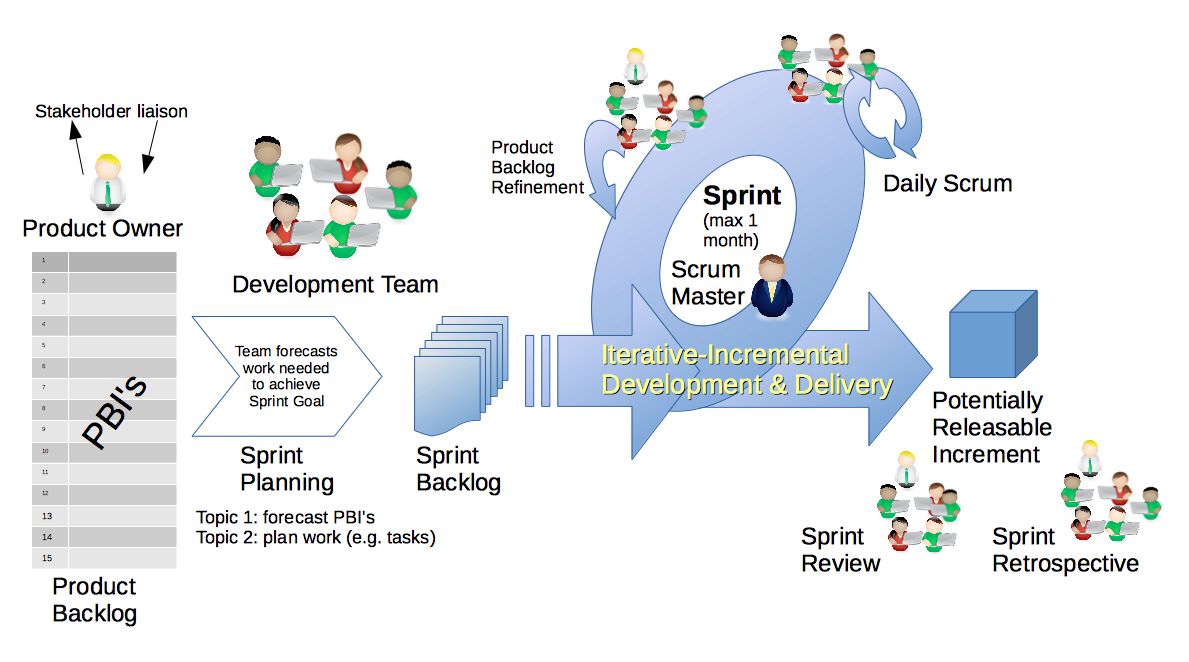
\includegraphics[scale=0.2]{scrum1.png} 
\caption{Metodolog�a Scrum}
\end{figure}

\end{frame}
\subsection{Iteraciones}

\begin{frame}\frametitle{Iteraciones} 

\begin{itemize}
\item \textbf{Iteraci�n 0}:Investigaci�n y aprendizaje
\item \textbf{Iteracion 1}:Primeras demos
\item \textbf{Iteraci�n 2}:A�adir interactividad
\item \textbf{Iteraci�n 3}:A�adir posibilidades de filtrado dimensional.
\item \textbf{Iteraci�n 4}: Creaci�n de la biblioteca
\item \textbf{Iteraci�n}: A�adir paneles y otras caracter�sticas.
\end{itemize}

\end{frame}

\section{Dise�o y resultados}

\subsection{Arquitectura}
\begin{frame}
\begin{figure}
  \centering
  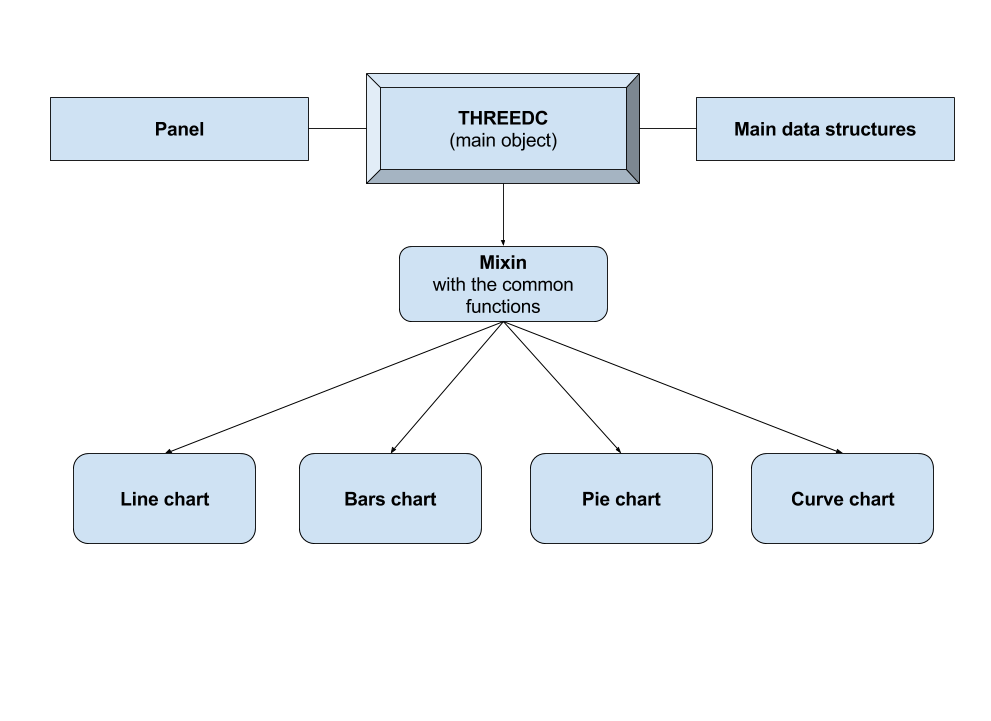
\includegraphics[width=10cm, keepaspectratio]{diagram.png}
  \caption{Arquitectura de la librer�a}
\end{figure}
\end{frame}
\subsection{Funciones principales}
\subsection{Tipos de gr�ficas}
\subsection{Filtros}
\subsection{Paneles}

\section{Conclusiones}
\subsection{Conocimientos aplicados}
\subsection{Lecciones aprendidas}
\subsection{Trabajos futuros}


\section{Referencias} 

\begin{frame}\frametitle<presentation>{Referencias}


\begin{thebibliography}{10}

\bibitem[Devlin, 2002]{Devlin}
A.J.~Chorin, J.E.~Marsden.
\newblock {\em A Mathematical Introduction to Fluid Mechanics}
\newblock Springer-Verlag, 1980.

\bibitem[Devlin, 2002]{Devlin}
K.~Devlin.
\newblock {\em The Millenium Problems. The Seven Greatest Unsolved Mathematical Puzzles of Our Time}
\newblock Basic Books, 2002.

\bibitem{Fefferman} 
C.~Fefferman.
\newblock {\em Clay Mathematics Institute, Millenium Problems. Official problem description}.
\newblock 
\href{http://www.claymath.org/millennium/Navier-Stokes\_Equations/}{http://www.claymath.org/millennium/Navier-Stokes\_Equation}
\bibitem[Wikipedia contributors, 200]{Wikipedia}
Wikipedia contributors
\newblock {\em Navier-Stokes equations}
\newblock Wikipedia, The Free Encyclopedia., 2008.
\newblock 
\href{http://en.wikipedia.org/wiki/Navier-Stokes\_equations}{http://en.wikipedia.org/wiki/Navier-Stokes\_equations}

\end{thebibliography}
\end{frame}


\end{document}